\subsubsection{Overview of File Structure}
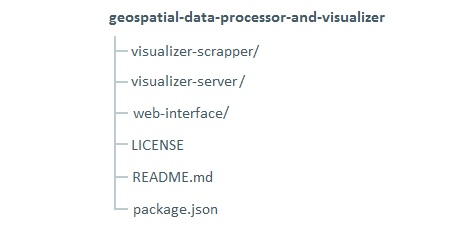
\includegraphics[width=\textwidth]{overall_file_structure} \\[0.5cm]
\begin{itemize}
	\item \textbf{visualizer-server} \\
	The back-end server, visualizer-server is git sub-module. This means that it is located in a different repository location entirely \href{https://github.com/Coeus2016/visualizer-server}{source}. After cloning the repository the developer may edit and add to the code as they wish. It runs a NodeJS server using ExpressJS 
	
	\item \textbf{web-interface}
	The front-end, visualizer-web-interface like the server is also a git sub-module. This means that it is located in a different repository location entirely \href{https://github.com/Coeus2016/visualizer-web-interface}{source}. After cloning the repository the developer may edit and add to the code as they wish. The current framework being used is AngularJS
\end{itemize}
